\begin{frame}[c]\frametitle{Data Sources}

To model general online human advice-seeking interactions, we chose to construct datasets from Reddit forums (subreddits) focused on advice.

\pause

\vspace{10mm}

\begin{table}[H]
    \centering
    \begin{tabular}{ll}
        \toprule
        \textbf{r/AskParents} & \textbf{r/needadvice} \\ \midrule
        parents seeking advice & a general advice forum \\ \midrule
        less moderation & more moderation\\ \midrule
        \multirow{3}{*}{no flairs} & 5 flairs -- ``Education'', ``Career'',\\
        & ``Mental Health'', ``Life Decisions'', \\
        & ``Friendships''\\ \bottomrule
    \end{tabular}
    \label{tab:datasources}
\end{table}

\end{frame}


\begin{frame}[c]\frametitle{Annotation}
    \begin{figure}
        \centering
        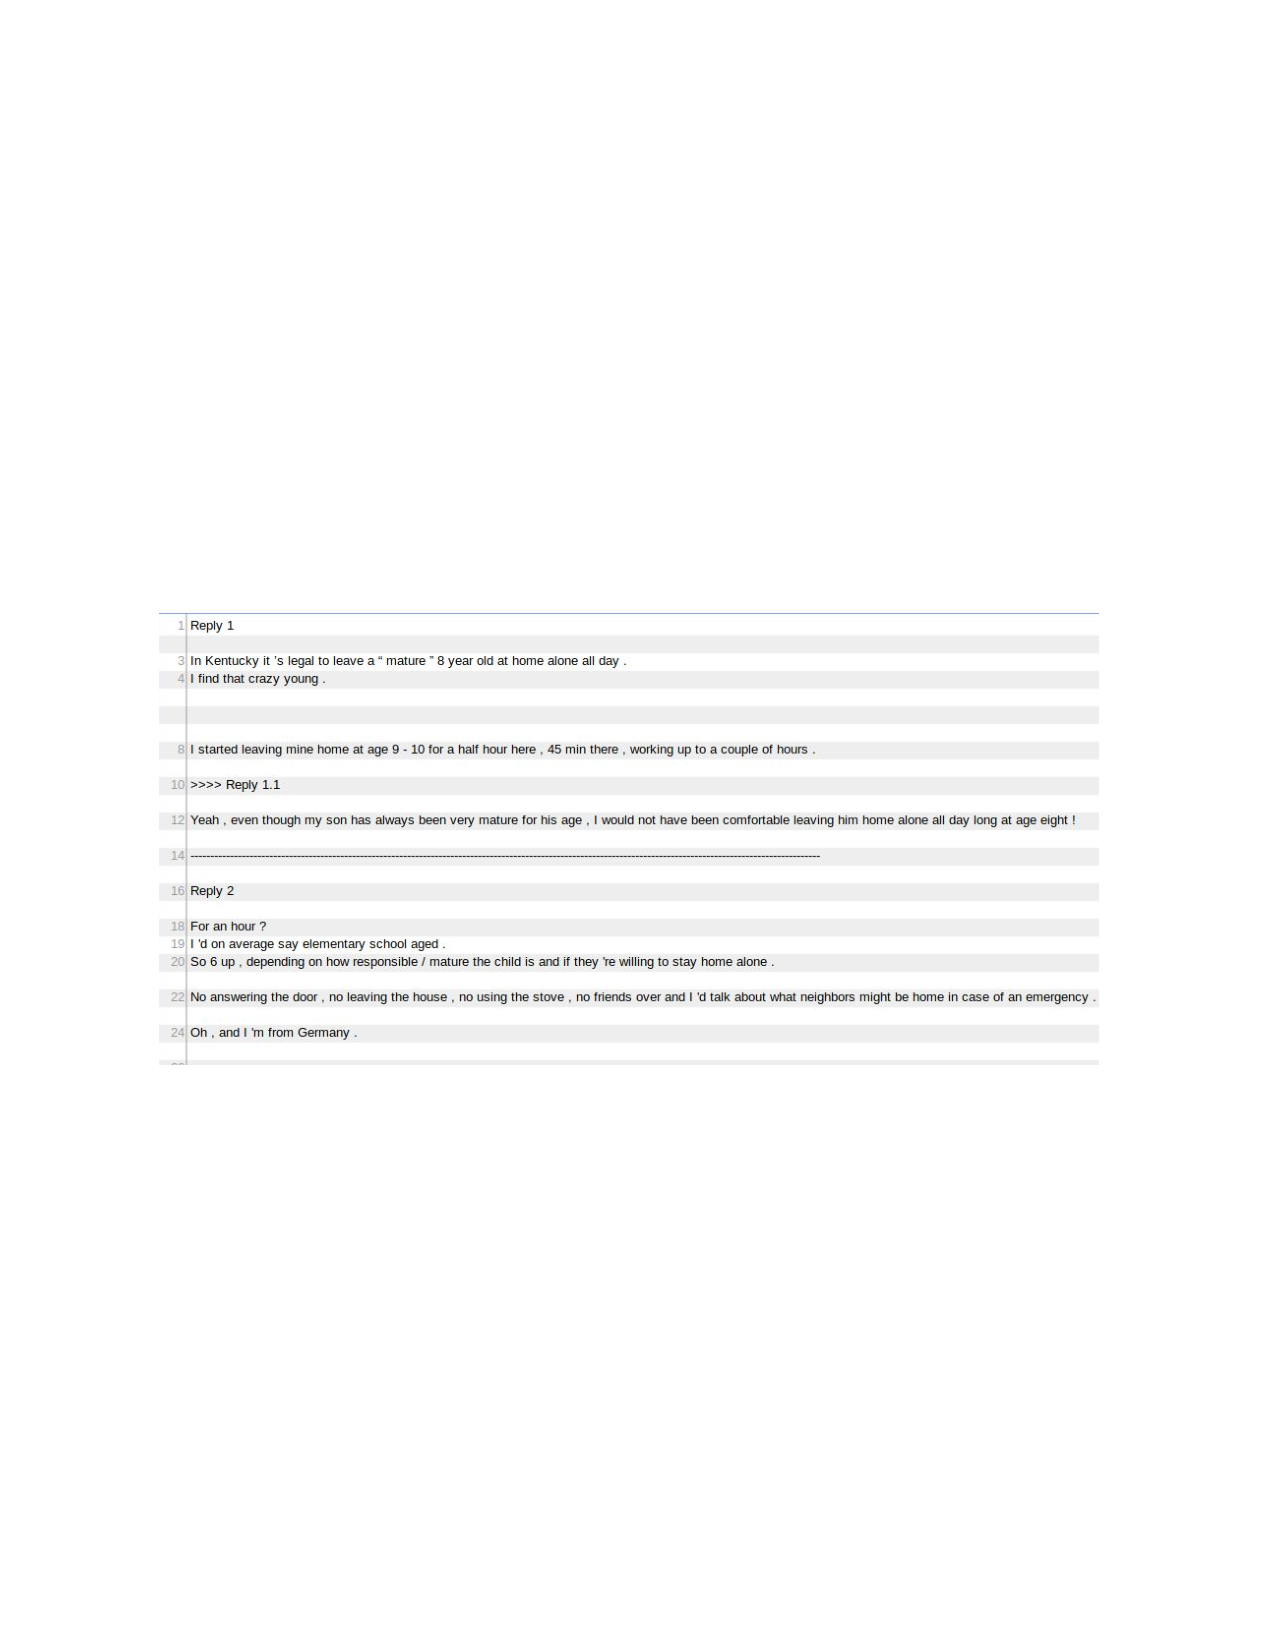
\includegraphics[width=\linewidth]{figures/ann-1.pdf}
        \caption{}
    \end{figure}
\end{frame}

\begin{frame}[c]\frametitle{Annotation}
    \begin{figure}
        \centering
        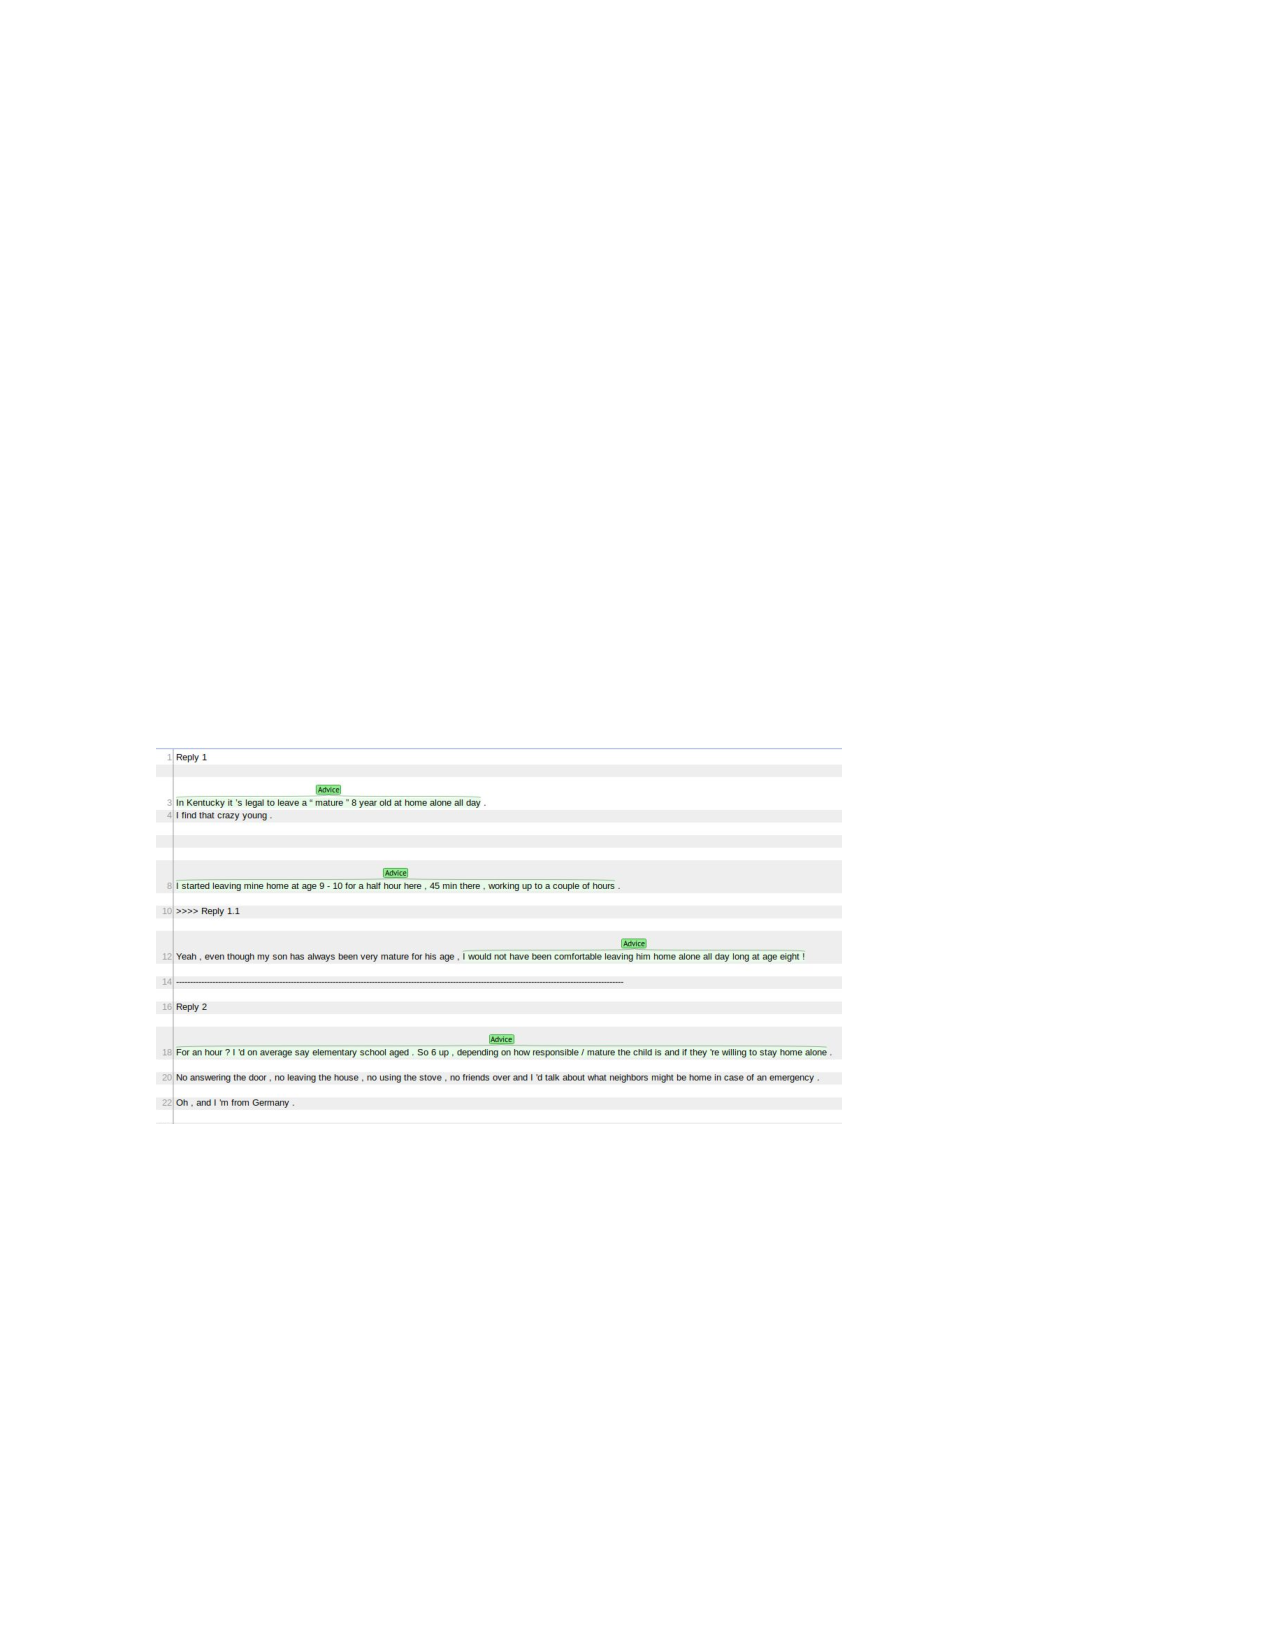
\includegraphics[width=\linewidth]{figures/ann-2.pdf}
        \caption{}
    \end{figure}

5 annotators on Amazon Mechanical Turk annotated each HIT of 5 comments.

\end{frame}


\begin{frame}[c]\frametitle{Label Aggregation}

We chose \textbf{sentences} as the units of advice.

How to aggregate sentence labels while accounting for inter-annotator variability?

\pause

\vfill

\begin{alertblock}{Dawid-Skene Labels}
        An EM based algorithm that estimates the label with the maximum estimated \textbf{posterior probability} by iteratively computing annotator competencies and type probabilities~\citep{dawid_maximum_1979}.
\end{alertblock}

\end{frame}


\begin{frame}[c]\frametitle{Dataset}
    \centering

    r/AskParents \quad 10,594 sentences \quad 407 posts

    r/needadvice \quad 7,862 sentences \quad 277 posts

    \vfill

    Data (and code) available at \href{https://github.com/venkatasg/Advice-EMNLP2020}{\sansc github.com/venkatasg/Advice-EMNLP2020}

\end{frame}

